\documentclass[11pt,a4paper]{article}

\usepackage[utf8]{inputenc}
\usepackage[T1]{fontenc}
\usepackage[english]{babel}
\usepackage[margin=2.0cm]{geometry}
\usepackage{parskip}
\usepackage{hyperref}
\usepackage{graphicx}
\usepackage{float}

\hypersetup{colorlinks=true,urlcolor=blue,linkcolor=black}
\setlength{\parskip}{0.45em}

\title{\vspace{-1.4cm}Final Reflection: AI Solution Sprint 2026}
\author{Tauheed Butt \\ \small \href{https://tauheed.dev}{tauheed.dev}}
\date{17 September 2026}

\begin{document}

\maketitle

\section*{What went well}

The part that went best for me was the actual development. Our team was given
the CareLoop challenge, which asked how you get people to keep coming back and
logging the maintenance and lifecycle of things they own, like home appliances,
instead of forgetting about a product the day after they buy it. We managed to
build a working answer to that in two days.

On the frontend I built the mobile app in React Native, and on the AI side I
built an agent using Vercel's AI SDK. I wired up LangFuse on top of it so we
could trace every call the agent made, see where it was slow, and see where it
was making the wrong call. Getting full telemetry working inside a two-day
sprint was not something I expected to pull off, but it worked end to end.

Beyond the build itself, the rest of the event went well too. The final
solution held together, the pitch came out clean, and the presentation to the
jury went the way we wanted. The team also worked well together across the two
days, which is not something I could take for granted going in, since half of
us had never worked together before.

\section*{What I can do better next time}

The thing I would change is when I start writing code. I lean heavily toward
writing specs before I touch implementation, and in a two-day sprint that habit
cost me time I did not have to spare. Specs are useful when the team is large
or the problem is unclear, but for a fast-moving hackathon build, spending too
long on the spec before anything runs is the wrong trade. Next time I want to
get a rough version working first and write the spec around what already
exists, rather than the other way around.

\section*{What I learned}

Most of what I learned was not about the AI stack itself, since I had touched
most of those tools before. It was about pitching and about working with
teammates who do not have a technical background. Part of our team came from
product and from sustainability, with no engineering experience, and figuring
out how to split work with them was its own problem to solve. It meant
learning how to hand off pieces of the build that did not need code at all,
like the framing of the pitch or the reasoning behind the product decisions,
and trusting that work as much as the engineering.

That also meant the sprint was not only a coding exercise. A large part of it
was product thinking: what to build, what to leave out, and how to explain why
those choices made sense to people who were not going to read the code.

\section*{How I will put this into practice}

The AI tooling is the most direct thing I can carry forward. I had researched
LLM tracing and observability before this sprint without ever wiring it into a
real product. Now that I have implemented LangFuse end to end, I know where it
breaks down and where it needs more work, and that is knowledge I only got
from actually shipping it under pressure. I plan to keep building agent-based
tools with this stack and treat this sprint as the first real version of that,
not a one-off.

The pitch itself is the other thing I am taking with me. Presenting our
solution to the jury in front of a room that size was new for me, and it went
well. That gives me more confidence to put myself forward for talks and
pitches going forward, rather than treating presenting as something to avoid.

\section*{How I used AI in this assignment}

I used Claude Code as a drafting tool. I gave it my own notes on each of the
four reflection questions, in my own words, and asked it to structure them
into a clear report. I reviewed and edited the resulting text myself, and the
thinking and conclusions in this report are my own.

\section*{Evidence: blog post}

I was heads down in development on the first day and forgot to post. To make
up for it, I wrote a full blog post on LinkedIn covering my journey across the
whole event, tagged \#AISolutionSprint:
\href{https://www.linkedin.com/pulse/ai-solution-sprint-another-hackathon-tauheed-butt-vaxaf/}{LinkedIn: AI Solution Sprint, Another Hackathon}.
Screenshots of the published post are below.

\begin{figure}[H]
  \centering
  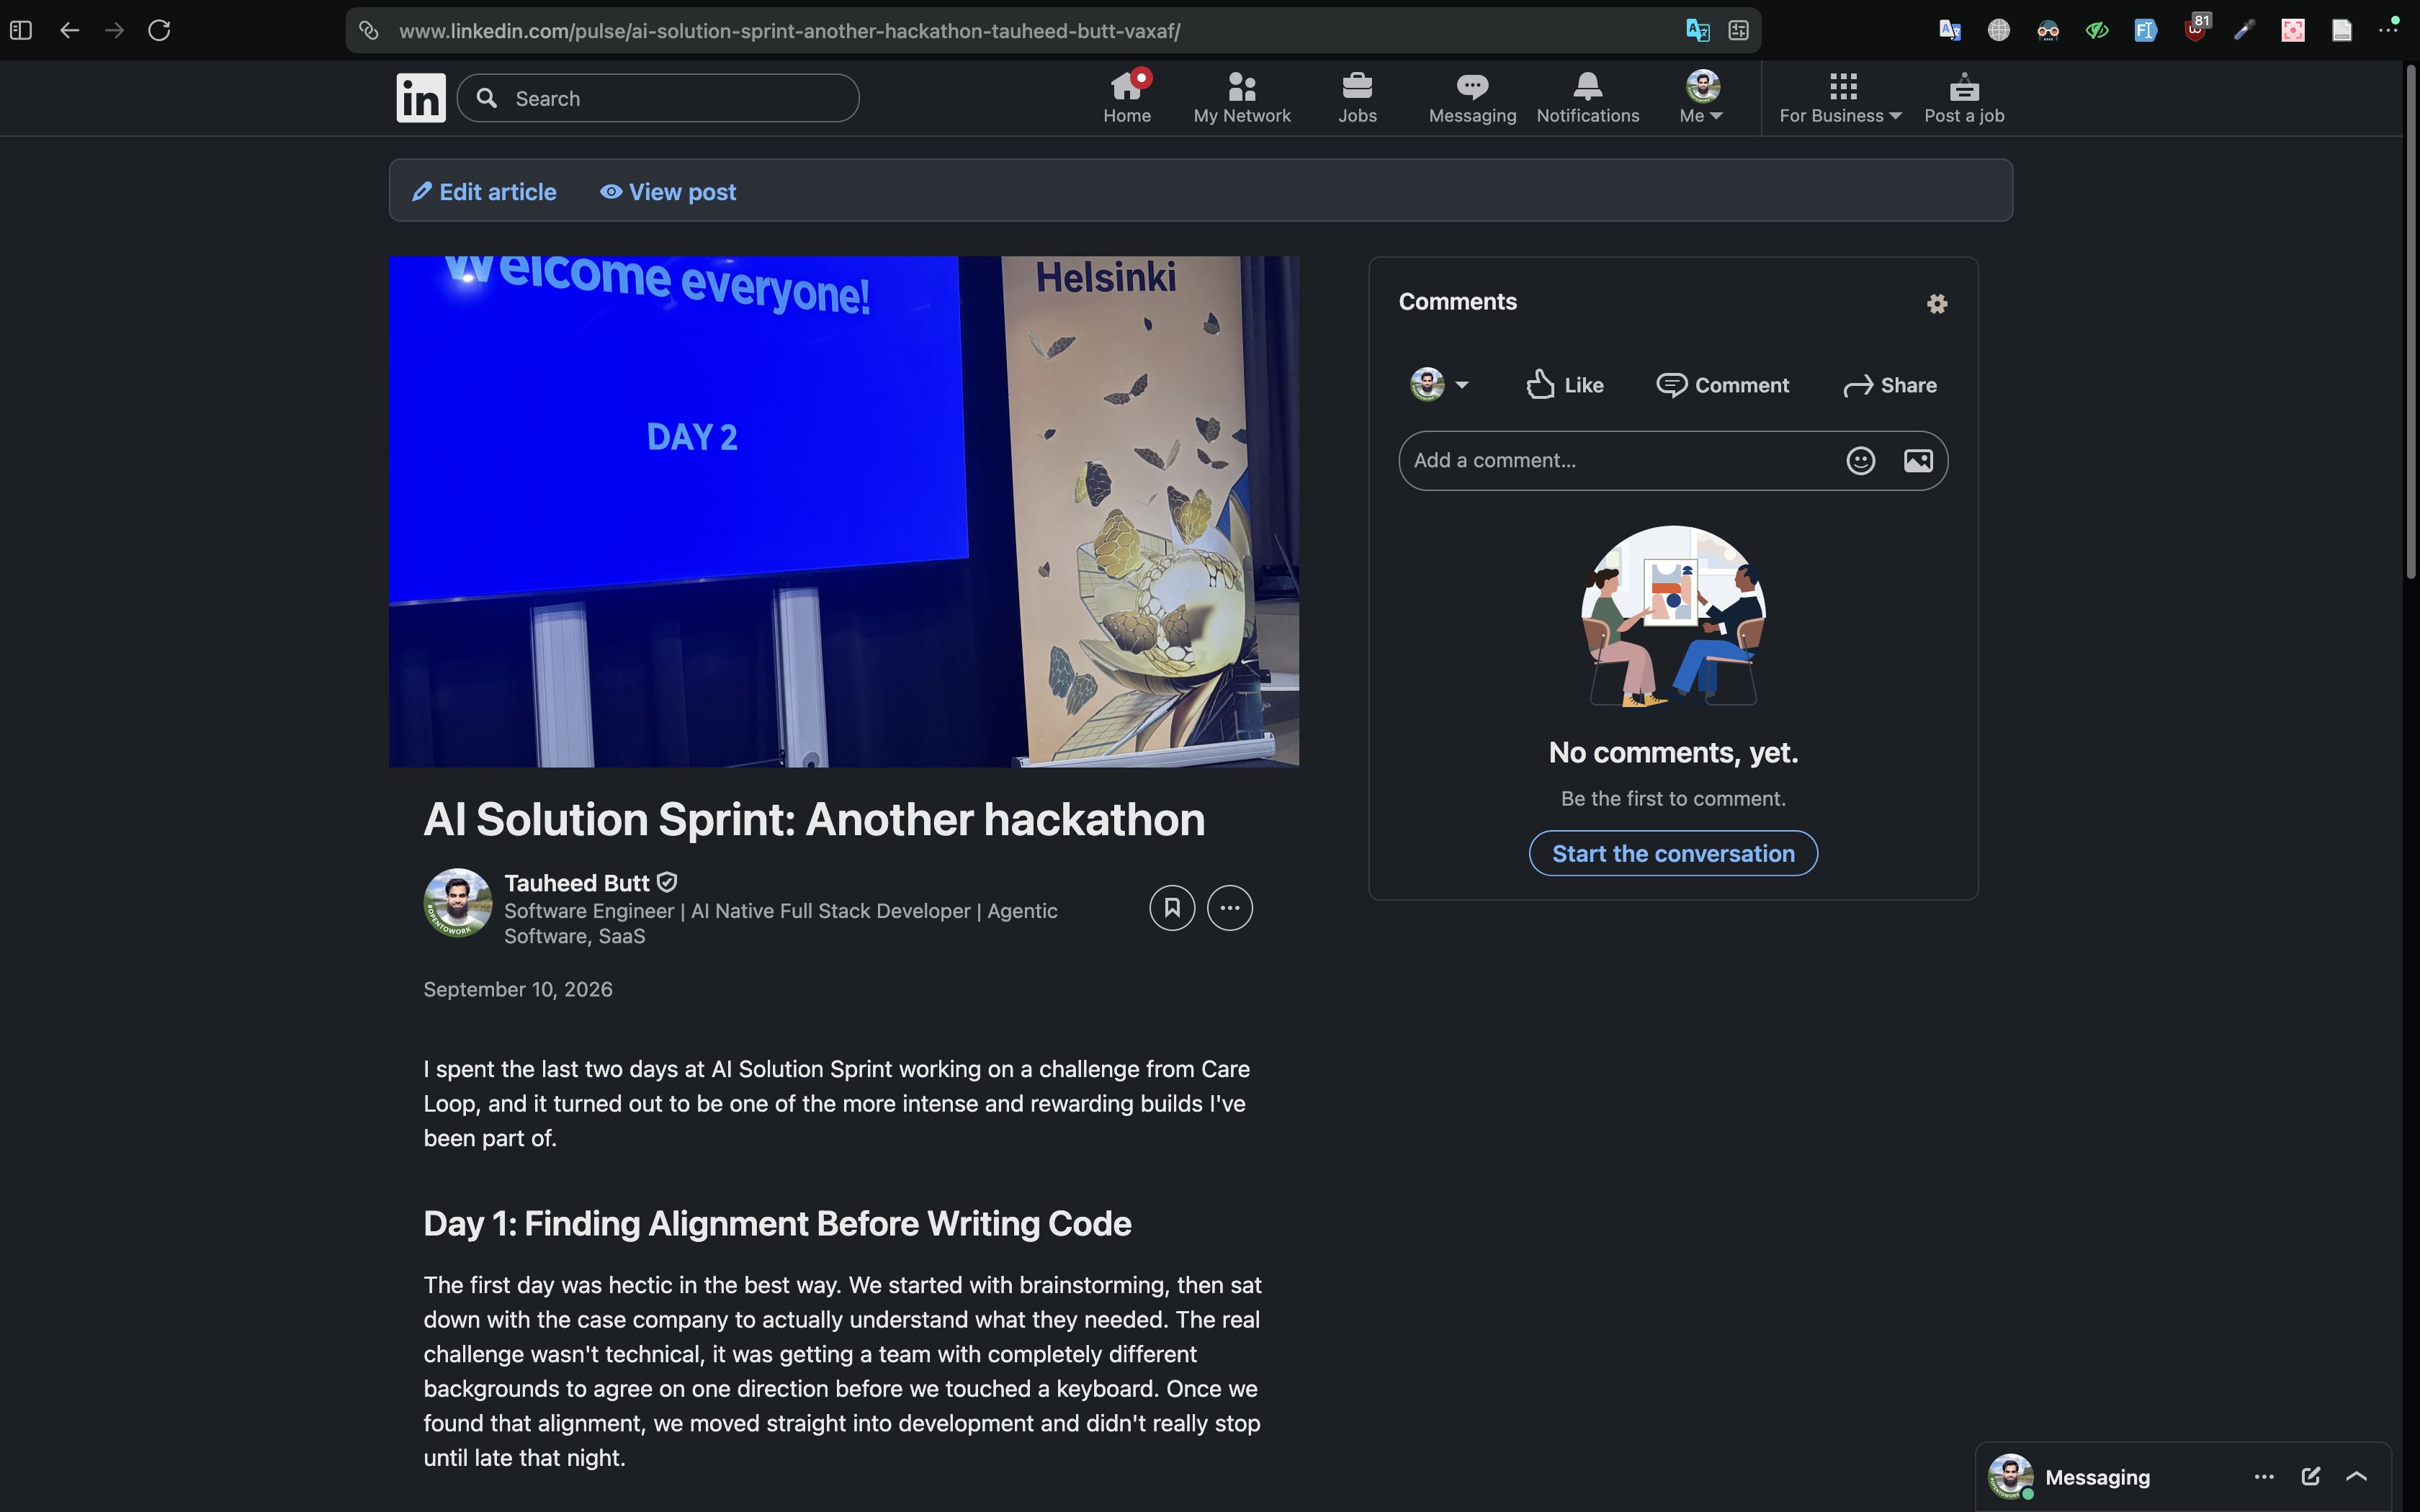
\includegraphics[width=0.85\textwidth]{images/blog-image-1.png}
\end{figure}

\begin{figure}[H]
  \centering
  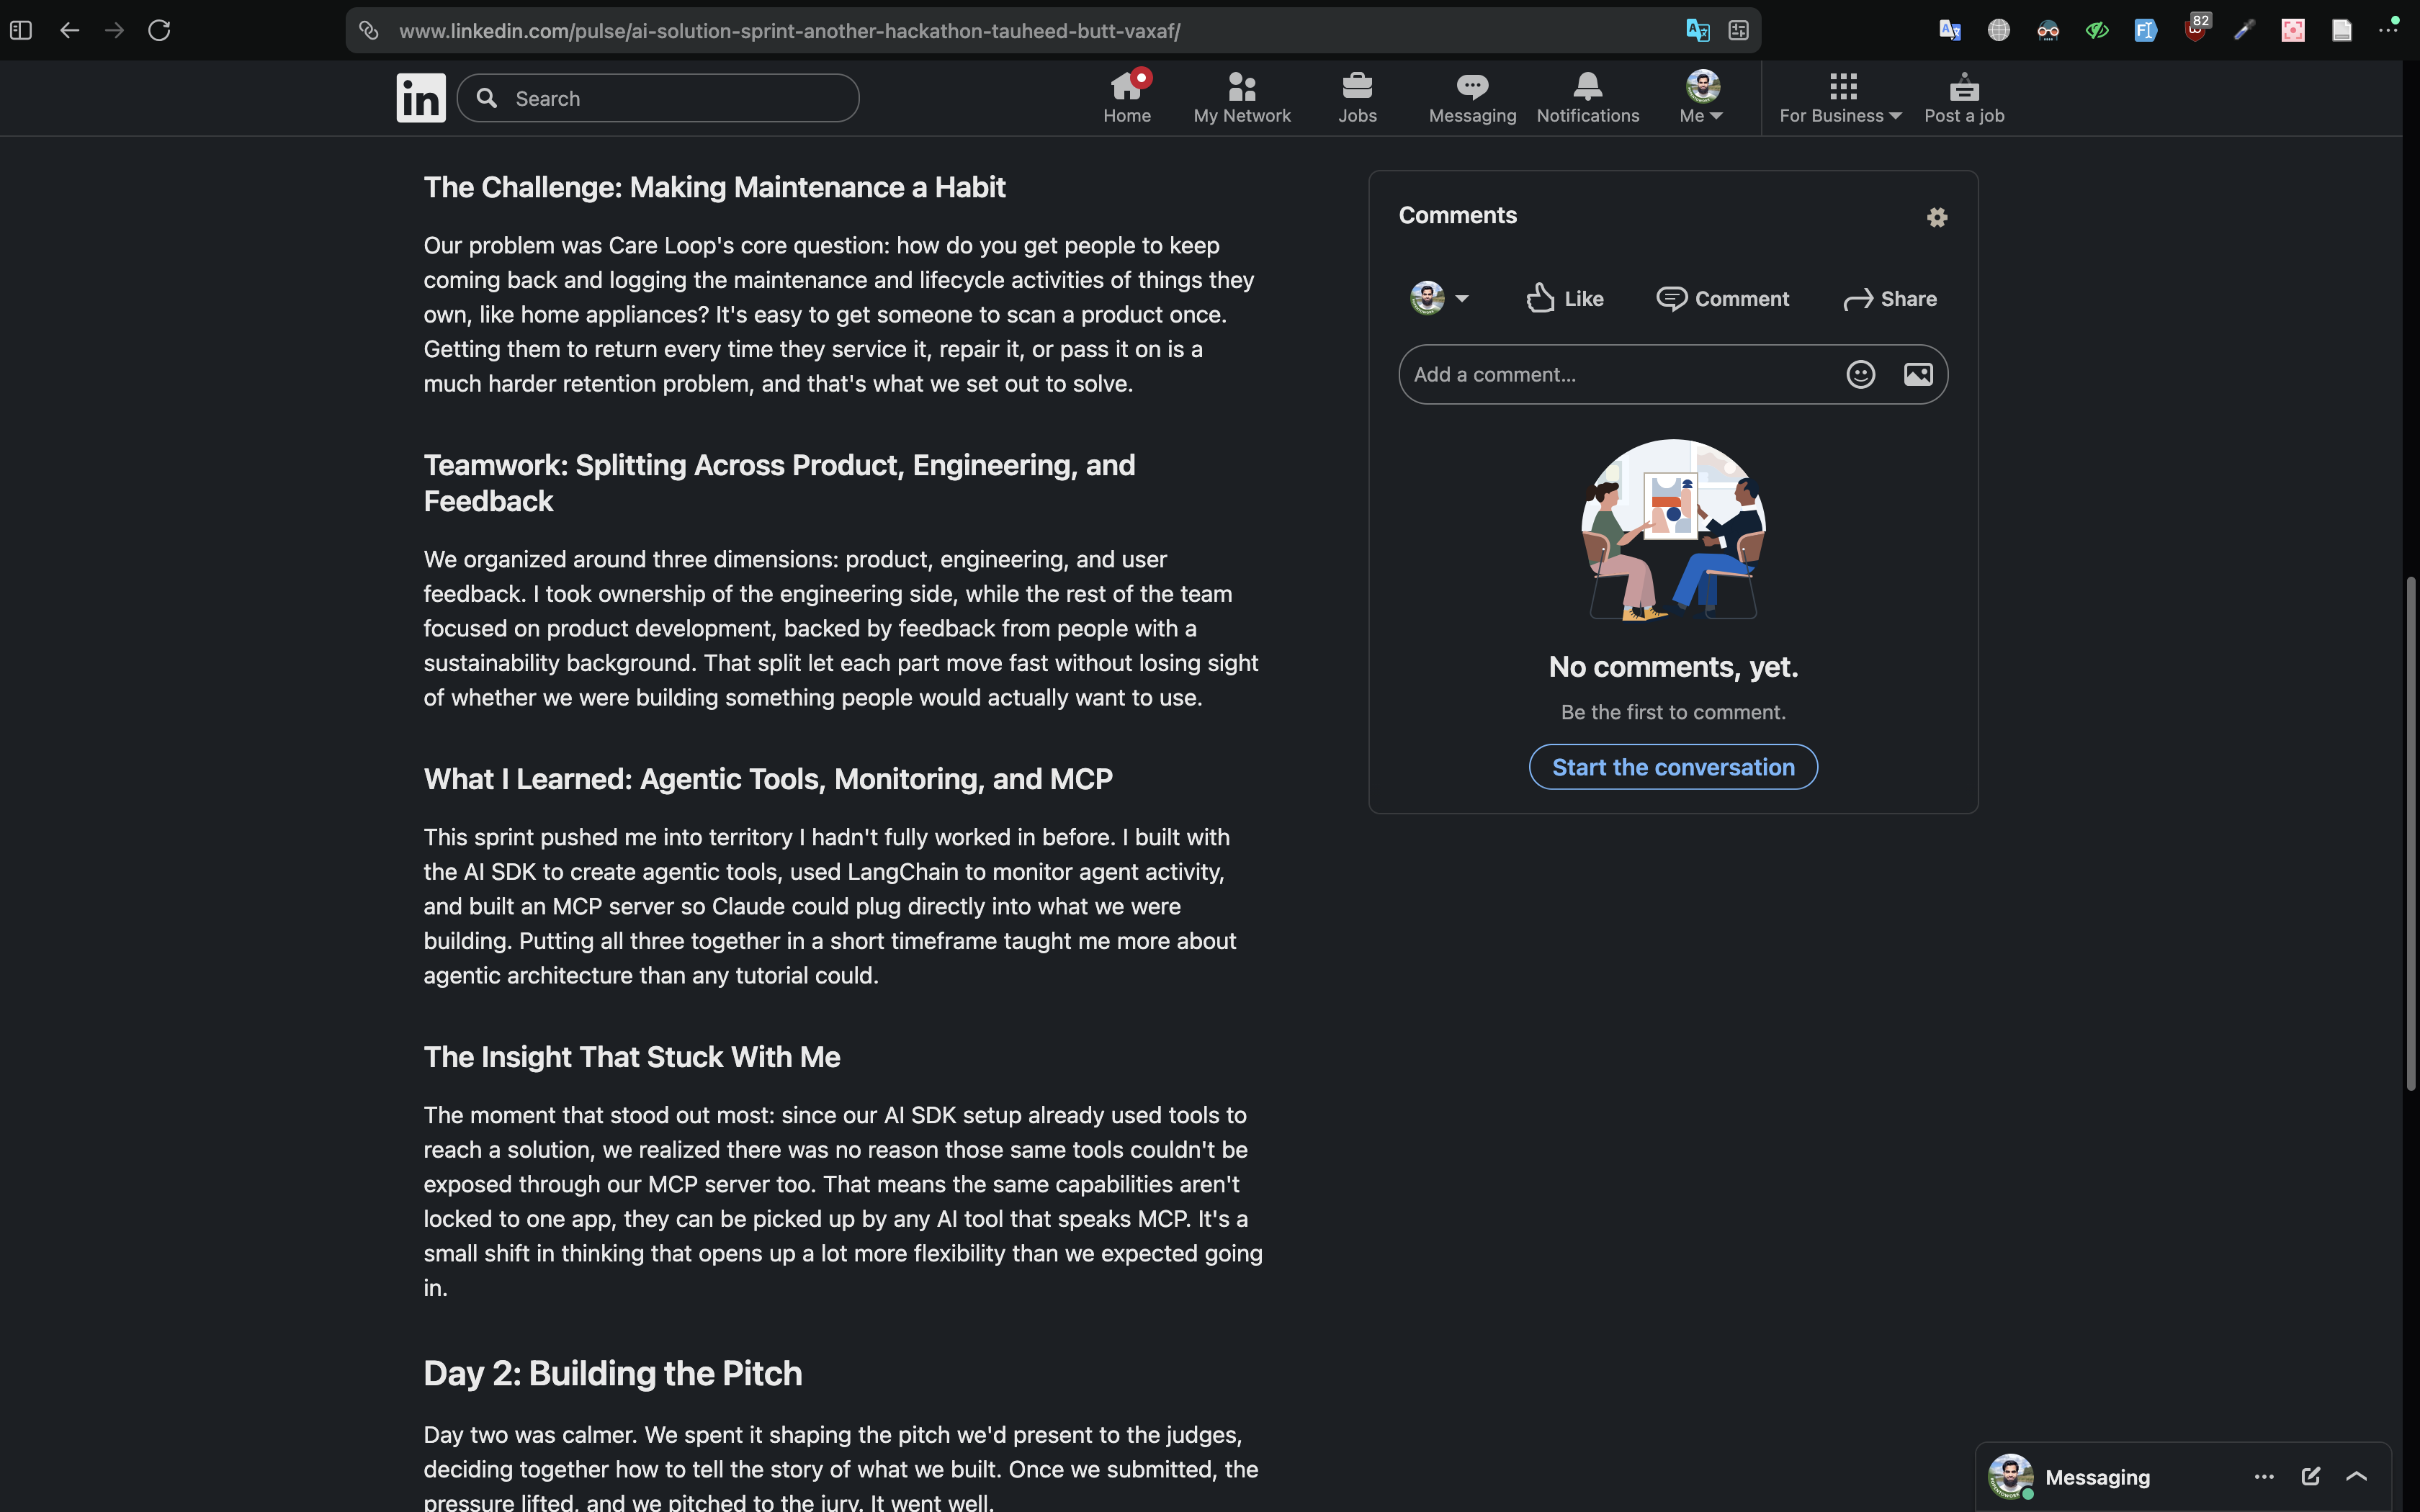
\includegraphics[width=0.85\textwidth]{images/blog-image-2.png}
\end{figure}

\begin{figure}[H]
  \centering
  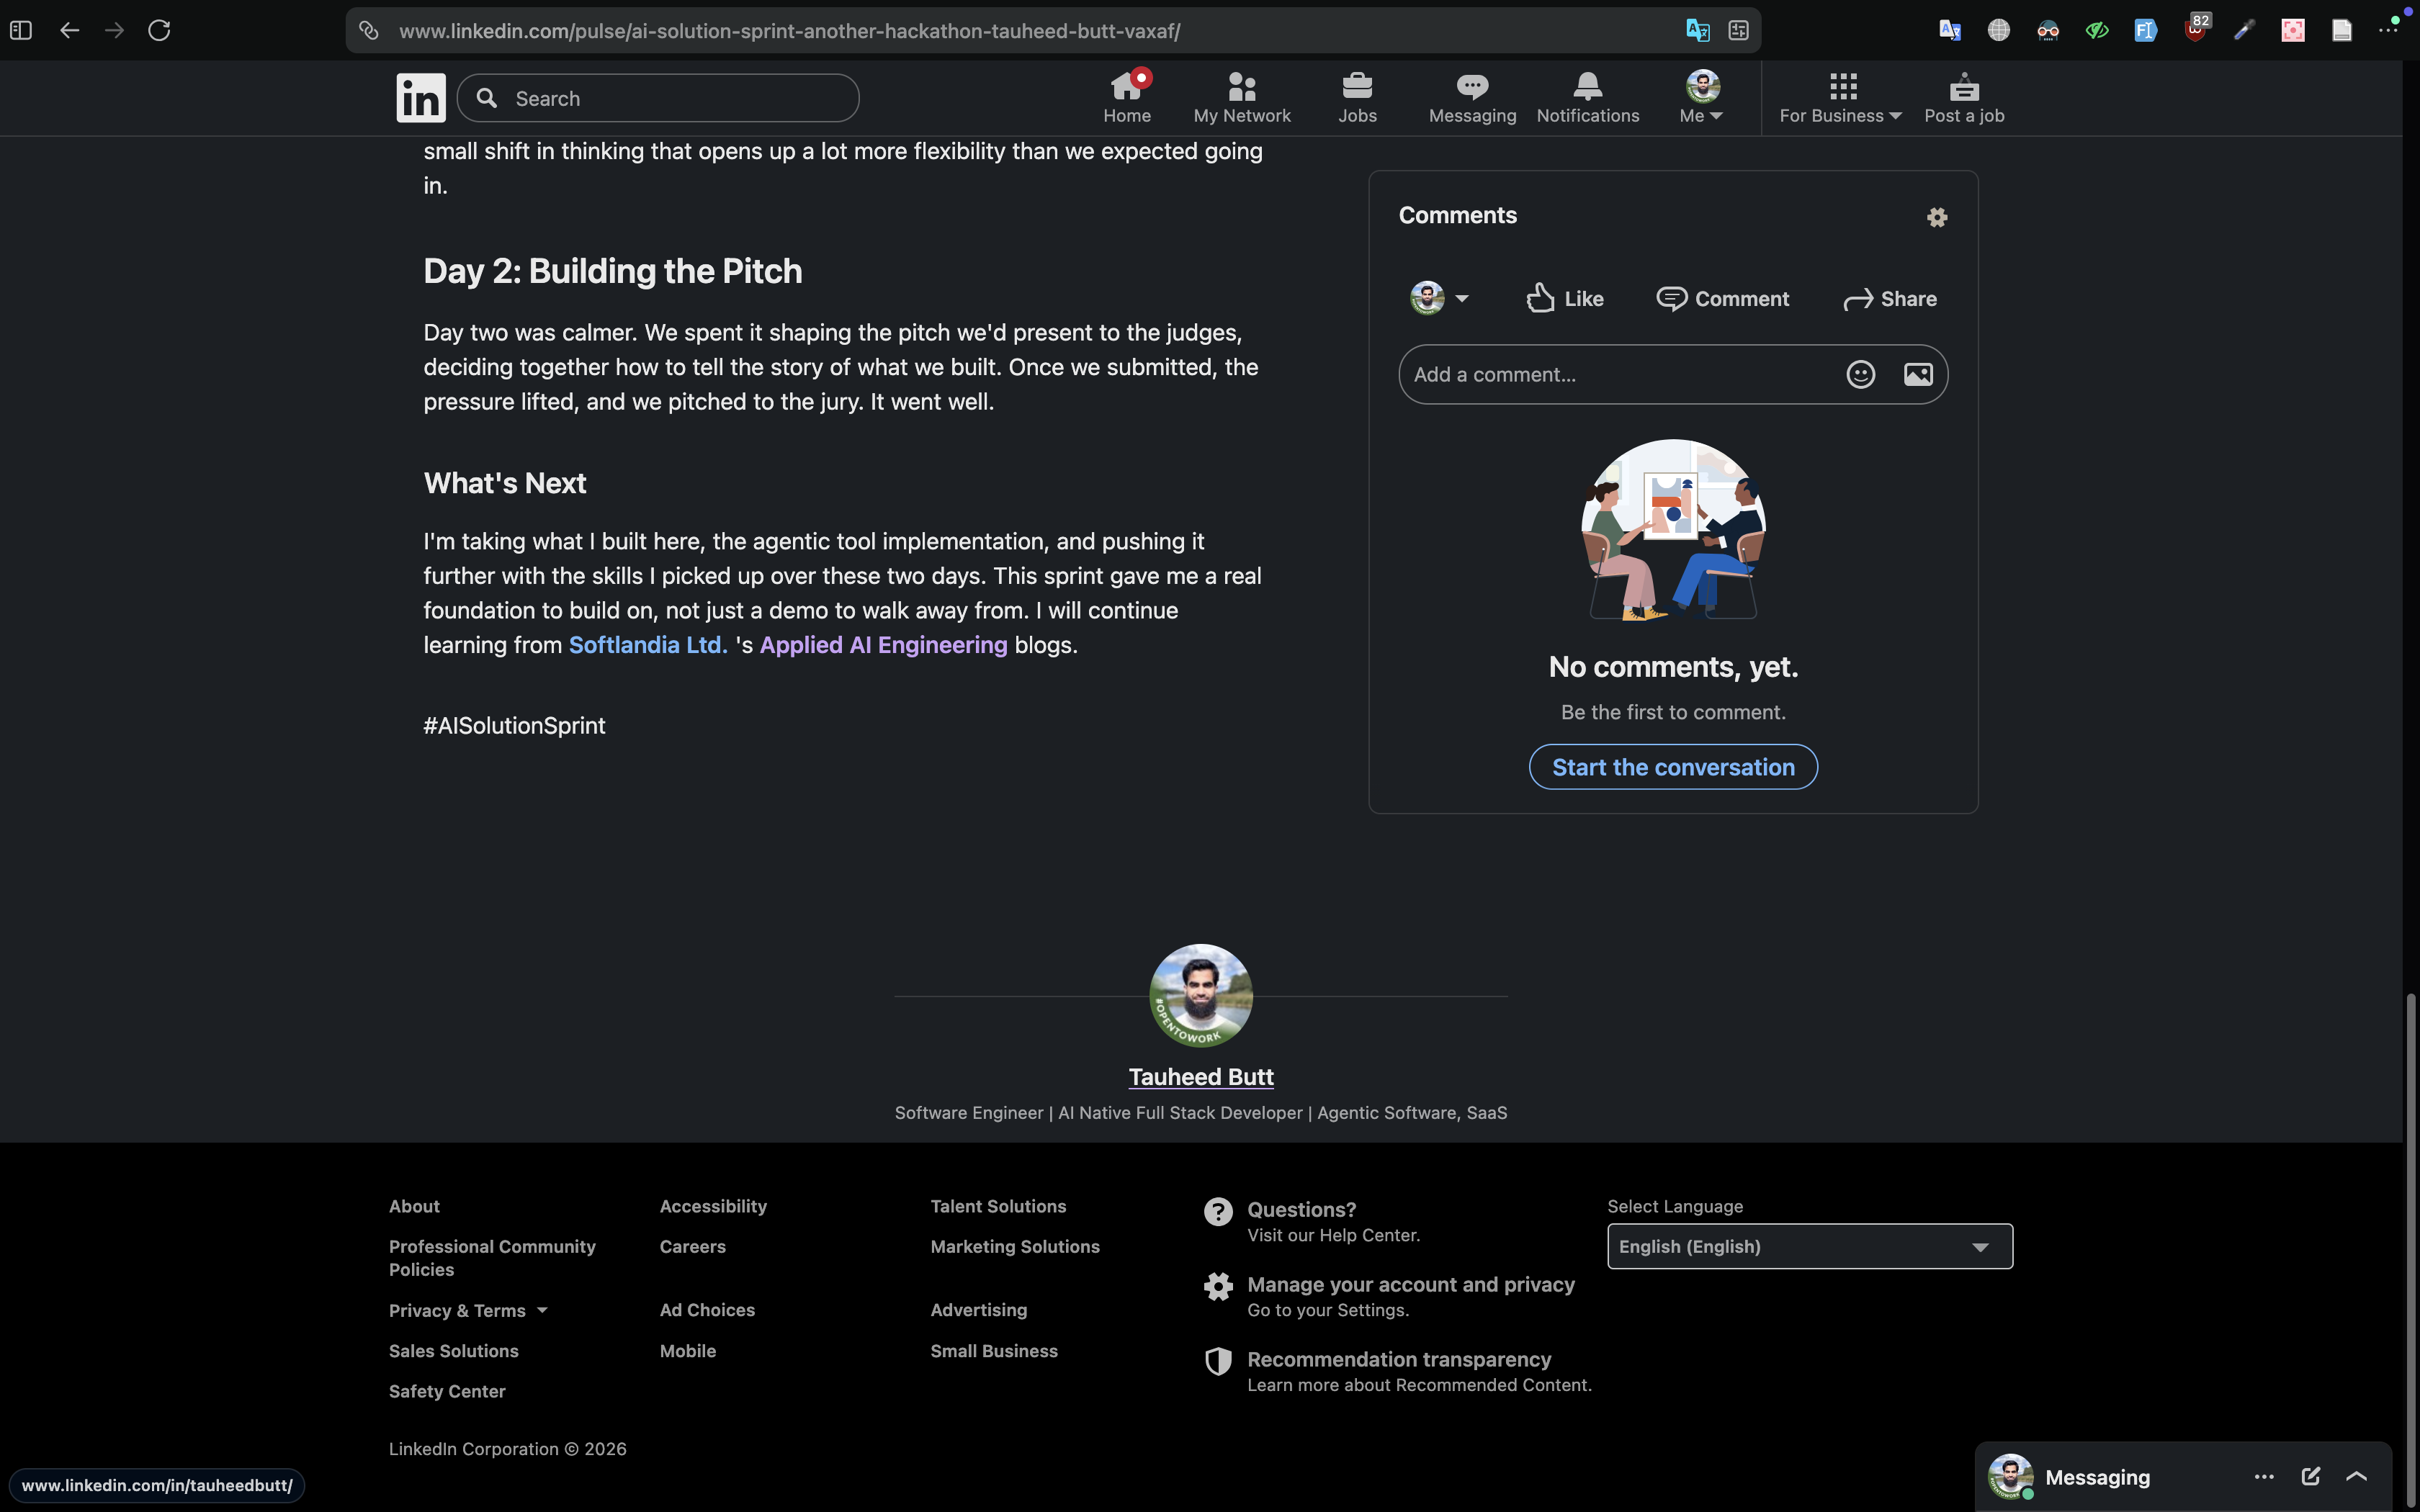
\includegraphics[width=0.85\textwidth]{images/blog-image-3.png}
\end{figure}

\end{document}
